% =====================================================================
%  PIANTA DEL LABORATORIO SISTEMI - DOMOTICA con le file A, B, C
%  Verifica del 23/10/2026, 3BETC, 25 studenti (30 postazioni: 5 vuote).
%  Imposta questo file come Main document e compila.
%  Regola: la fila è (colonna + fila del banco) mod 3, così chi è accanto
%  o davanti/dietro ha sempre una fila diversa.
% =====================================================================
\documentclass[a4paper,11pt]{article}
\usepackage{stili/comune}
\usepackage[scaled=0.92]{helvet}
\renewcommand{\familydefault}{\sfdefault}
\usepackage[a4paper,margin=1.5cm]{geometry}
\pagestyle{empty}
% \posto{x}{y}{numero postazione}{contenuto}{vuota se vuota}
\newcommand{\posto}[5]{%
  \ifstrequal{#5}{vuota}%
    {\draw[thick,dashed,fill=black!6] (#1,#2) rectangle ++(2.4,1.9);}%
    {\draw[thick] (#1,#2) rectangle ++(2.4,1.9);}%
  \node[font=\scriptsize,anchor=north] at (#1+1.2,#2+1.85) {Postazione #3};
  \node at (#1+1.2,#2+1.0) {#4};
  \ifstrequal{#5}{vuota}{}{\draw[thin] (#1+0.2,#2+0.3) -- (#1+2.2,#2+0.3);}}
\begin{document}
\begin{center}
{\Large\bfseries Laboratorio Sistemi -- Domotica \quad\textmd{|}\quad Classe 3BETC\par}
\vspace{2pt}{\large Verifica di Sistemi Automatici del 23/10/2026 -- disposizione delle file A, B, C\par}
\vspace{8pt}
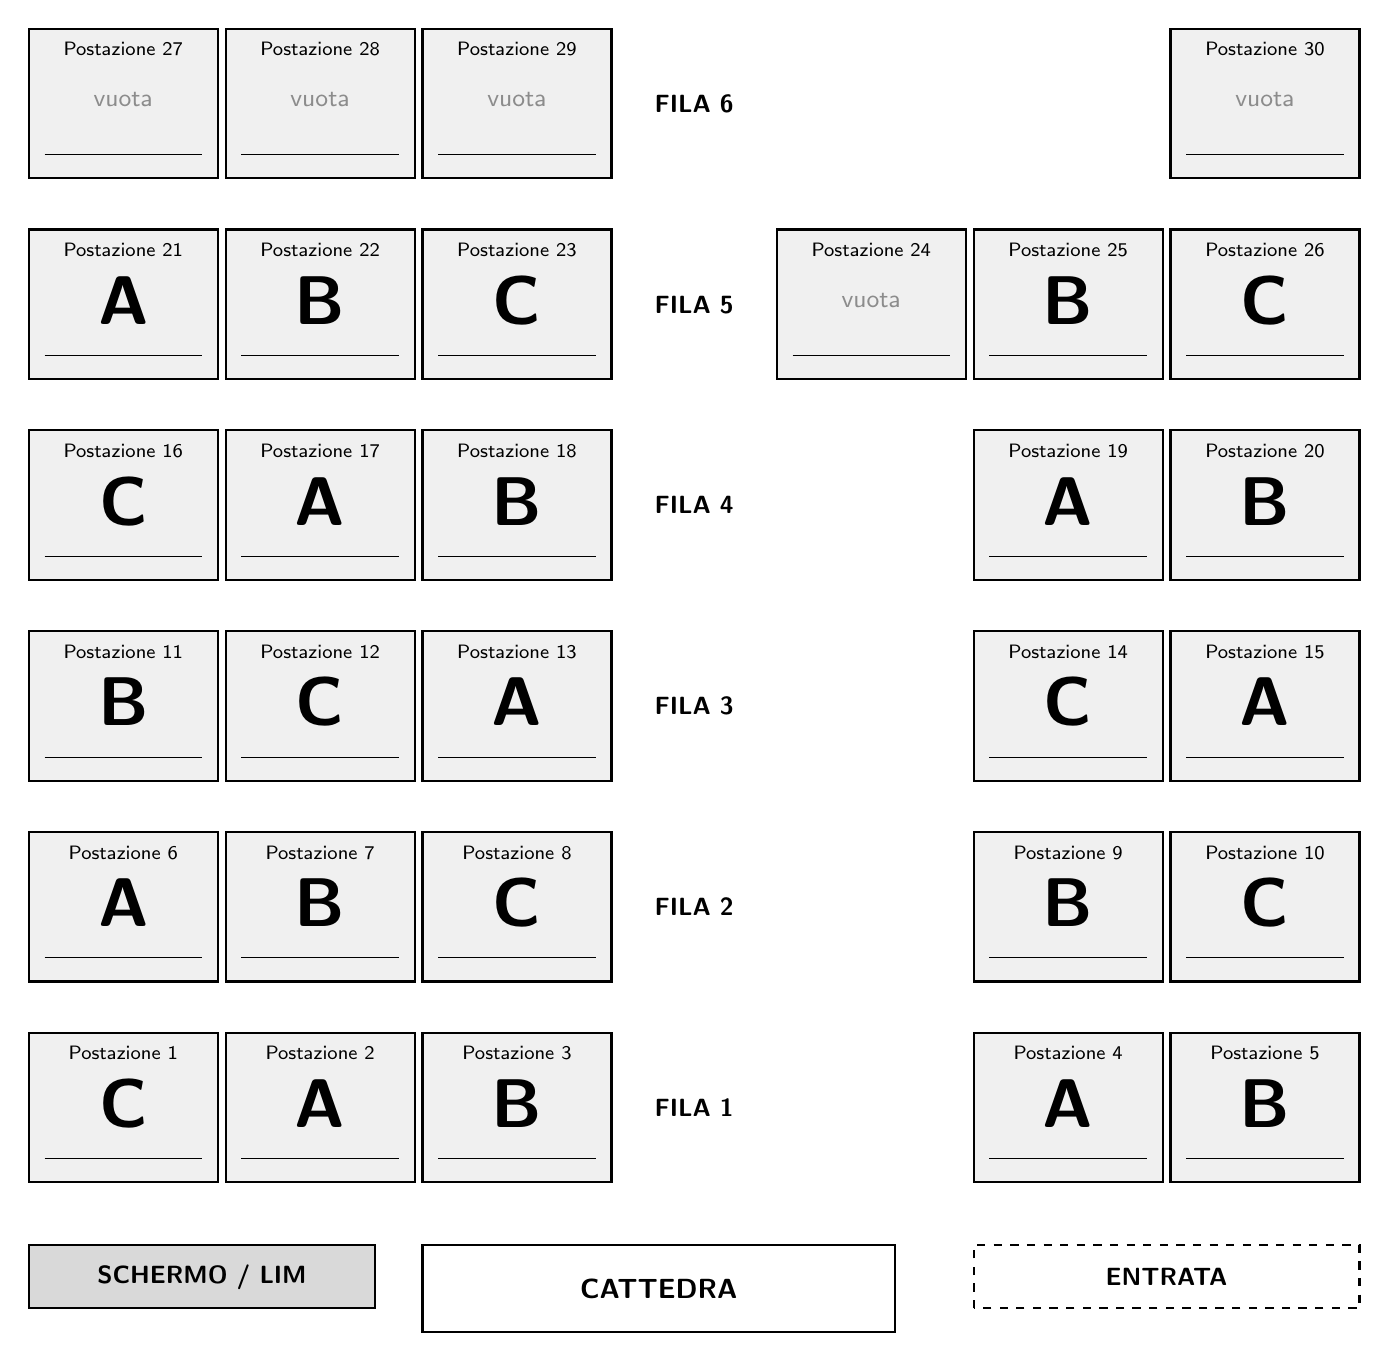
\begin{tikzpicture}[x=1cm,y=1cm,scale=1.0,transform shape]
  \posto{0}{0.0}{1}{\fontsize{26}{28}\selectfont\bfseries C}{}
  \posto{2.5}{0.0}{2}{\fontsize{26}{28}\selectfont\bfseries A}{}
  \posto{5}{0.0}{3}{\fontsize{26}{28}\selectfont\bfseries B}{}
  \posto{12}{0.0}{4}{\fontsize{26}{28}\selectfont\bfseries A}{}
  \posto{14.5}{0.0}{5}{\fontsize{26}{28}\selectfont\bfseries B}{}
  \posto{0}{2.55}{6}{\fontsize{26}{28}\selectfont\bfseries A}{}
  \posto{2.5}{2.55}{7}{\fontsize{26}{28}\selectfont\bfseries B}{}
  \posto{5}{2.55}{8}{\fontsize{26}{28}\selectfont\bfseries C}{}
  \posto{12}{2.55}{9}{\fontsize{26}{28}\selectfont\bfseries B}{}
  \posto{14.5}{2.55}{10}{\fontsize{26}{28}\selectfont\bfseries C}{}
  \posto{0}{5.1}{11}{\fontsize{26}{28}\selectfont\bfseries B}{}
  \posto{2.5}{5.1}{12}{\fontsize{26}{28}\selectfont\bfseries C}{}
  \posto{5}{5.1}{13}{\fontsize{26}{28}\selectfont\bfseries A}{}
  \posto{12}{5.1}{14}{\fontsize{26}{28}\selectfont\bfseries C}{}
  \posto{14.5}{5.1}{15}{\fontsize{26}{28}\selectfont\bfseries A}{}
  \posto{0}{7.6499999999999995}{16}{\fontsize{26}{28}\selectfont\bfseries C}{}
  \posto{2.5}{7.6499999999999995}{17}{\fontsize{26}{28}\selectfont\bfseries A}{}
  \posto{5}{7.6499999999999995}{18}{\fontsize{26}{28}\selectfont\bfseries B}{}
  \posto{12}{7.6499999999999995}{19}{\fontsize{26}{28}\selectfont\bfseries A}{}
  \posto{14.5}{7.6499999999999995}{20}{\fontsize{26}{28}\selectfont\bfseries B}{}
  \posto{0}{10.2}{21}{\fontsize{26}{28}\selectfont\bfseries A}{}
  \posto{2.5}{10.2}{22}{\fontsize{26}{28}\selectfont\bfseries B}{}
  \posto{5}{10.2}{23}{\fontsize{26}{28}\selectfont\bfseries C}{}
  \posto{9.5}{10.2}{24}{\textcolor{black!45}{\small vuota}}{vuota}
  \posto{12}{10.2}{25}{\fontsize{26}{28}\selectfont\bfseries B}{}
  \posto{14.5}{10.2}{26}{\fontsize{26}{28}\selectfont\bfseries C}{}
  \posto{0}{12.75}{27}{\textcolor{black!45}{\small vuota}}{vuota}
  \posto{2.5}{12.75}{28}{\textcolor{black!45}{\small vuota}}{vuota}
  \posto{5}{12.75}{29}{\textcolor{black!45}{\small vuota}}{vuota}
  \posto{14.5}{12.75}{30}{\textcolor{black!45}{\small vuota}}{vuota}
  \node[font=\small\bfseries] at (8.45,0.95) {FILA 1};
  \node[font=\small\bfseries] at (8.45,3.5) {FILA 2};
  \node[font=\small\bfseries] at (8.45,6.05) {FILA 3};
  \node[font=\small\bfseries] at (8.45,8.6) {FILA 4};
  \node[font=\small\bfseries] at (8.45,11.149999999999999) {FILA 5};
  \node[font=\small\bfseries] at (8.45,13.7) {FILA 6};
  % lato cattedra
  \draw[thick,fill=black!15] (0,-1.6) rectangle ++(4.4,0.8) node[midway] {\small\bfseries SCHERMO / LIM};
  \draw[thick] (5,-1.9) rectangle ++(6,1.1) node[midway] {\bfseries CATTEDRA};
  \draw[thick,dashed] (12,-1.6) rectangle ++(4.9,0.8) node[midway] {\small\bfseries ENTRATA};
\end{tikzpicture}
\end{center}
\vspace{4pt}
\begin{center}\small
\renewcommand{\arraystretch}{1.3}
\begin{tabular}{|c|c|l|}\hline
\textbf{Fila} & \textbf{Studenti} & \textbf{Postazioni}\\\hline
A & 8 & 2, 4, 6, 13, 15, 17, 19, 21\\\hline
B & 9 & 3, 5, 7, 9, 11, 18, 20, 22, 25\\\hline
C & 8 & 1, 8, 10, 12, 14, 16, 23, 26\\\hline
Vuote & 5 & 24, 27, 28, 29, 30\\\hline
\end{tabular}
\end{center}
\end{document}
